\chapter{Experiments}\label{ch:experiments}
In order to answer the research question posed by this thesis, a series of experiments was conducted using \benchmark to evaluate and compare three agents of increasing complexity: a do-nothing agent, a greedy agent, and a trainable \ac{ppo} agent. Rather than testing a single grid configuration, the experiments cover a broad range of scenarios, including unmodified standard test grids, intentionally destabilised topologies, gradually intensified stress conditions, and pure performance tests. This enables a general ranking of the agents to be obtained, as well as a detailed analysis of their individual strengths and weaknesses across different metrics and categories.

The chapter is structured into three main parts. Section \ref{sec:experiment_setup} describes the experimental setup, including the selected scenarios, the configuration of the benchmark categories, the two baseline agents and the custom PPO agent, as well as the expectations derived from this setup. Section \ref{sec:experiment-results} then presents the results obtained from running all experiment scenarios, first providing an overall comparison and then breaking the results down by experiment category. Finally, Section \ref{sec:exp-analysis-interpretation} analyses and interprets these results in depth. It explains recurring patterns in the agents' behaviour and summarises the findings into a strength and failure profile for each agent.

\section{Experimental Setup}\label{sec:experiment_setup}
This section describes the setup used to conduct the experiments in this thesis. Section \ref{ssec:experiment-scenarios} first introduces the experiment categories and the specific scenarios contained within them, along with the configuration of the benchmark's category weights. Section \ref{ssec:baseline-agents} then presents the two baseline agents used in all experiments, the do-nothing and greedy agents presented in Section \ref{sec:agent-integration}, together with the defined reward function that is used in the experiments. Section \ref{ssec:custom-agent-setup} then describes the architecture, training process and tuning of the custom \ac{ppo} agent, which is compared against the two baselines. Finally, Section \ref{ssec:exp-expectation} formulates the expected outcomes for each experiment category based on the experiment design decisions presented in this section.

\subsection{Experiment Scenarios}\label{ssec:experiment-scenarios}
The experiments cover different fields important in grid stability and operation. All the experiments are categorised into two groups. The \textbf{grid operation} experiments range from a normal run of unmodified IEEE grids, to diverse scenario coverage by different grid modifications and finally to a stress test, where difficulty is increased by multiple levels of scaling of a grid modification. The category of \textbf{performance-only} contains one experiment, which compares runtimes and computational resource usage between agents.

\subsubsection{General Setup}
Each of the experiments is run with a whole day as episode length. Using the data from SimBench as profiles, this gives 96 iterations for one episode, as the time series values are provided for every 15 minutes. It is important to note that although SimBench provides profiles for renewable generation as well, only conventional generation and load profiles are used throughout the experiments in this thesis. This choice was made to isolate the effect of the individual grid modifications discussed in Section \ref{ssec:implementation-grid-mod} on the agents' performance, without introducing the additional, weather-driven variability and intermittency associated with renewable generation. Furthermore, while SimBench also provides larger and more complex power grids, the grids used in this chapter were deliberately chosen to be less complex. This decision allows for a clearer overview of the agents' behaviour, as larger grids would be considerably more difficult to visualise and present within the scope of this thesis.

For all experiments, the 14-bus and 30-bus IEEE test cases are used as power grids. Figure \ref{fig:exp-grids} shows the two power grids, following the visual conventions introduced in Section \ref{ssec:implementation-grid-profiles}, and highlights the grid components that are modified in the experiments. In the figures, buses are drawn as small circles, while substations are drawn as bigger circles. Furthermore, it is visible that the 30-bus grid does not contain any transformers. The difference in size between the two grids is also visible from the figures, as the 30-bus grid has significantly more components, forming a more complex, interconnected grid than the 14-bus one.

Table \ref{tab:cat-weights-setup} shows the chosen weights of each benchmark category used for the evaluation of each experiment. For the grid operation experiments, the focus is on grid stability, hence \textit{computational performance} is left out of the evaluation. As for the performance-only experiment, the focus is opposite to that of the grid operation experiments, with only the \textit{computational performance} category being evaluated.

\begin{table}[htbp]
    \centering
    \caption{Benchmark Category Weights}
    \label{tab:cat-weights-setup}
    \begin{tabular}{lcc}
        \hline
        Category & Grid Operation & Performance-only \\
        \hline
        Overload Mitigation & 2 & 0 \\
        Voltage Violation Mitigation & 2 & 0 \\
        Survival & 3 & 0 \\
        Costs & 1 & 0 \\
        Computational Performance & 0 & 1 \\
        \hline
    \end{tabular}
\end{table}


\subsubsection{Chosen Scenarios and Experiments}
For each scenario, challenging test days are identified following the steps in Section \ref{sec:evaluation-protocol}. This was done by finding profile days on which the do-nothing agent achieves a benchmark score of about 50 and the greedy agent scores lower, i.e. days where neither inaction nor the locally optimal action suffices for a high score. The benchmark score is set up with the category weights shown in Table \ref{tab:cat-weights-setup}, using the weights from grid operation. In the following paragraphs the exact scenario selection process is explained. Table \ref{tab:scenarios-setup} shows all chosen scenarios over every experiment. It also explains which profile days were used and which grid components were modified. 

\paragraph{Standard Analysis.}
The first experiment category looks at the standard 14-bus and 30-bus from the IEEE test cases. This test shows the first overall comparison between the agents, with a normal power grid that does not have any extremes or modifications. It compares the performance in normal grid operation. As seen in Table \ref{tab:scenarios-setup} under the scenarios \textit{14B\_ORIG} and \textit{30B\_ORIG}, for the 14-bus grid, three profile days were chosen, and for the 30-bus grid, one profile day was chosen. For the 14-bus grid there were more challenging scenarios, while the unmodified 30-bus grid did not have many difficult days, so the one with the lowest benchmark score was chosen.

\paragraph{Diverse Scenario Coverage Analysis.}
This experiment explores how \benchmark can be used, to cover more diverse scenarios. With grid modification, different cases in the 14- and 30-bus power grids are created. This experiment examines how the agents behave with more extreme cases, where there is a factor making the grid less balanced and adding instability to it. 

One case in this experiment is the shifting of the generation of power more towards a single generator. This makes one generator produce more energy, while the others produce less. Another case shifts the consumption more to a single load to create a less balanced grid. For both generation and load scaling the sum of generation or consumption is preserved to the value in the original power grid. If generation or consumption is concentrated at a single point, larger, unevenly distributed power flows result, which make the grid less robust to withstand disturbances and making stabilisation more difficult.
To find the right trials, each one of the generators and loads from the grids in the 14- and 30-bus IEEE test case has been scaled in separate experiments. Finally, the generator and load with the biggest impact on destabilising the grid have been selected for this experiment. This has been done again like in Section \ref{sec:evaluation-protocol}, using the scores of the two baseline agents. The chosen generators and loads and how much they are scaled are noted in Table \ref{tab:scenarios-setup} and their position in the grid is highlighted in Figure \ref{fig:exp-grids}.

The other cases of grid modification focus on limiting power grid components for the grid with 30 buses. The modifications include maintenance events in generation or transmission lines, or downscaling the capacity of transmission lines.
The transmission lines, that had the highest loading during the standard unmodified network runs, have been chosen to be downscaled or put under maintenance. By limiting or disabling these bottleneck components of the power grid, the power needs to be redirected into other lines, testing the agent's ability to plan when components have issues. In the case of the generator maintenance, the generator near the external grid has been put into maintenance. As a result, the external grid has to be used much more. The problem is that the generator under maintenance is connected to four lines, while the external grid is only connected to two lines, making it a bigger challenge to supply the power without overloading the lines. For these modifications again Table \ref{tab:scenarios-setup} documents the chosen components and Figure \ref{fig:exp-grids} shows their location in the grid.

\paragraph{Stress-Test Analysis.}
For this experiment category, the scalable scenarios from the diverse scenario experiment are used. For each of the cases, different levels of scaling are evaluated, increasing the difficulty of each power grid gradually. Each of these tests contains three levels of scaling. First, a light scaling modifies the grid just slightly, affecting the difficulty very little. The next scaling uses exactly the same trials shown in the second experiment, which is right in the middle between the light and heavy scaling. For the heavy scaling the difficulty is increased the most, making it very hard to maintain a stable power grid. The scalable scenarios include the load, generator and line capacity modification tests. These trials test how each agent reacts to increasing stress, and if the different scaling of difficulty affects the scoring system. The exact scaling levels are documented in Table \ref{tab:scenarios-setup}, which shows for each scaling level the exact multiplier.

\paragraph{Performance Analysis.}
For this experiment the same scenarios as the standard analysis experiments are chosen. In this experiment, only the computational performance of the greedy and \ac{ppo} agents is evaluated. It tests the runtime and computational resource usage of both agents, working with the 14- and 30-bus grid. The goal is to illustrate, how these two agents compare in performance, measuring this on two different grid sizes, which hold different degree of complexity in connected components. 


\subsection{Baseline Agents}\label{ssec:baseline-agents}
As already covered, the experiments contain different categories that cover diverse scenarios to do a deep analysis. Each of these is evaluated and compared across multiple agents, always using the same three agents. 
The do-nothing agent is a reference point that indicates how demanding a scenario is without intervention. In some cases, the current network topology does not need much or any changes, as the power grid stays stable. 
But in more complex cases, like imbalanced power generation or demand, or bottleneck components that overload quickly, an agent that acts and changes the topology is needed. The greedy agent is chosen as a second baseline agent. It evaluates the available topology actions and chooses the one that yields the highest reward. 
For the reward, the customisable reward discussed in Section \ref{sec:agent-integration} is utilised. It punishes non-convergence in the power grid with a negative reward and looks at the metrics of maximal line loading and the present number of overloaded lines, both in $N-0$ power flow. The exact values set for the experiment are seen in Table \ref{tab:reward_settings}. The reward is deliberately kept simple and focuses only on two objectives, reducing line overloads in $N-0$ and avoiding non-convergence. Other metrics are intentionally excluded, even though \benchmark evaluates them. This allows the experiments to show how a narrow reward definition affects the benchmark scores. 

\subsection{Custom Agent Setup}\label{ssec:custom-agent-setup}
Choosing the best action for the current step is not always ideal. The best action for the current state might not be the best action for the stability of the grid. Both baseline agents do not have any component that plans for the future timesteps. In more complex power grids, an agent that is trained for its topology and profile can be more advantageous. For this reason, the third agent is a custom agent, implemented also as a test on how to use \benchmark as a developer, and to see how trained agents would compare to other untrained agents like the do-nothing and greedy agents.

The chosen custom agent is a \ac{ppo} agent that uses a \ac{gnn} as a policy encoder. It is implemented in RLlib as a subclass of the RayAgent described in Section \ref{sec:agent-integration} and follows the PPTopoGym reference agent \cite{pptopogym}. The encoder consists of a configurable stack of GINEConv layers, i.e. the edge-feature-aware variation of the \ac{gin} \cite{ginPaper}, which aggregates the embeddings of neighbouring nodes together with features of the connecting edges through a sum operation followed by an \ac{mlp} \cite{ginePaper}. The depth and width of the GINEConv layers are selected during hyperparameter optimisation for each scenario. These layers process the node features (voltage magnitude and angle at buses) and edge features (line and transformer loadings) of the power grid graph \cite{pptopogym}. As a result, each bus of the power grid is represented by an embedding generated by the GINEConv layers. The bus embeddings are then aggregated into a single embedding representing the entire power grid using a configurable graph-pooling operation, which is also selected during hyperparameter optimisation. Finally, the graph embedding is passed through a neural network with two heads, which create two outputs. The first head produces the action logits, which give one preference score for each action from the action space. The higher the score, the more preferable the action is for the grid state. During training, an action is sampled from the resulting probability distribution to encourage exploration, whereas during evaluation the action with the highest score is selected. The second head returns a value estimate, predicting the expected cumulative reward from the current state onwards.

The hyperparameters cover the architecture of the \ac{gnn} encoder and the fully connected head as well as the algorithmic parameters of \ac{ppo}, such as batch sizes, learning rate and clipping parameters. A complete listing and description of the parameters is given in Table \ref{tab:ppo-hparams}. Their optimisation is implemented using a customised child class of the OptunaTuner, presented in Section \ref{sec:agent-integration}. For each scenario the agent is first tuned over multiple trials and then trained with the tuned hyperparameters for a maximum of 3000 iterations, with early stopping if the best mean episode reward does not improve for 1000 consecutive iterations. Table \ref{tab:training-results} shows the results of the training for each scenario. The values shown are measured from the average cumulative reward over a full episode for the best training iteration. As each episode has 96 timesteps and the reward function per timestep has a maximum of one, the highest achievable cumulative reward is 96. As the penalty for non-convergence is -2, this is also the lowest cumulative reward. In some scenarios the \ac{ppo} agent almost reached the highest cumulative reward and in general the agent performed well in the 30-bus scenarios. In the 14-bus scenarios, however, it got some high values and some low values, even one close to the worst possible cumulative reward (for the highly scaled generator). 

\ac{ppo} is an established algorithm for grid topology control that combines naturally with a \ac{gnn} encoder. This allows the agent to exploit the topology of the power grid rather than operating on a flattened state vector. Training on individual load and generation profile episodes enables the agent to learn a policy that maps the current grid state directly to a switching action. This means that at runtime, the policy can directly decide one action. By contrast, greedy agents must simulate every candidate action at every time step to find the one with the highest reward. This makes the greedy agent slower and more computationally heavy during runtime. 

\subsection{Experiment Expectations}\label{ssec:exp-expectation}
Since the scenarios have been selected so that the greedy agent scores lower than the do-nothing agent, the relative ordering of the two baselines is fixed by design. Adding the custom agent introduces an additional element to the comparison: the effect of preparation through training. As the \ac{ppo} agent is tuned and trained to select actions that take future value into account, it is expected to achieve higher scores than both baseline agents. In simpler scenarios where the baselines already perform well, this difference is likely to be small. However, in more complex scenarios, the anticipatory behaviour of the \ac{ppo} agent should provide a clear advantage. As the reward only covers $N-0$ overloading and non-convergence, the agent is expected to excel in these two metrics in particular.

In the cost category, the metrics that evaluate executed actions are expected to favour the do-nothing agent, since an agent that never intervenes incurs no switching costs. However, this is just an advantage for this category, rather than an indication of effective operation. The outcome between the greedy agent and the \ac{ppo} agent is less clear. The greedy agent re-evaluates all candidate actions at every time step, so it may switch frequently. A trained policy, on the other hand, is more likely to settle into a stable topology and maintain it, resulting in lower costs. However, the reward used for training contains no cost component, so the \ac{ppo} agent has no motivation to minimise the number of actions and may act just as frequently as the greedy agent.

As for the grid modifications, they are expected to make grid stability more challenging to achieve, resulting in lower overall scores. The stress tests should gradually increase in difficulty across the scaling levels. While this increase should be reflected in the benchmark scores, the scores are not expected to drop in direct proportion to the amount of scaling. This is partly because only individual components are modified. As long as the surrounding lines still provide sufficient reserve capacity, the grid can absorb the additional stress to a degree, with few changes in the measured metrics. 

Finally, the decision-making process of the \ac{ppo} agent is expected to be faster than the action selection process of the greedy agent. As discussed in Section \ref{ssec:custom-agent-setup}, the greedy agent must compute the expected reward for each available action at each time step, whereas the policy of the PPO agent can choose an action directly. This advantage is expected to be more significant in the 30-bus grid, where the larger action space increases the number of required power flow calculations. However, the overall cost of the \ac{ppo} agent merely shifts into the preceding tuning and training phase.











\section{Results}\label{sec:experiment-results}
After running all the scenarios shown in the previous section, each agent has produced a set of scores for every scenario. This section presents these results, following the two experiment categories introduced in Section \ref{ssec:experiment-scenarios}. Section \ref{ssec:grid-operation-results} starts with an overall comparison of the total and category scores across all grid operation scenarios, before breaking the results down by the three individual experiments within this category: the standard test, the diverse scenario test and the stress test. It concludes with a look at the individual metric scores, to obtain a more granular view of the agents' performance. The performance-only experiment is then presented separately in Section \ref{ssec:perf-test-result}, comparing the runtime, CPU and memory usage of the greedy and \ac{ppo} agents across both tested grid sizes.

\subsection{Grid Operation Results}\label{ssec:grid-operation-results}
Table \ref{tab:agent_comparison} showcases the total score over all trials and their average category scores. Looking at the general overview, the \ac{ppo} agent achieved the highest scores, with the do-nothing agent having the second highest. The greedy agent on the other hand got lower scores in total. When looking at each category, the \ac{ppo} agent got higher scores than the other agents in all categories, except the costs category, where the do-nothing agent had the best score. Figure \ref{fig:bus-scores} documents the average category scores for the two power grids used in the experiments. Generally the scores are higher in the 30-bus grid. By contrast, for the costs category the \ac{ppo} agent and for the overload mitigation the do-nothing and greedy agents reach higher scores in the 14-bus grid.

\agentresulttable
  {Comparison of the agents in the grid operation experiments using the total score and category scores}
  {tab:agent_comparison}
  {
    Total Score & 58.20 & 41.25 & \textbf{64.86} \\
    \midrule
    Overload Mitigation & 53.90 & 51.44 & \textbf{73.22} \\
    Voltage Violation Mitigation & 41.54 & 30.21 & \textbf{56.85} \\
    Survival & 70.60 & 41.44 & \textbf{71.87} \\
    Costs & \textbf{62.89} & 42.34 & 43.09 \\
  }

Figure \ref{fig:exp-heatmap} offers a more detailed view over all trials, where the category scores of each agent for all the tested scenarios are shown. In general one can see that the agents achieved higher scores on average in the scenarios, where the 30-bus power grids were used. It is also visible, that the greedy agent has lower scores in general. Furthermore in the scenario with higher power generation scaling of generator 0 in the 14-bus grid, no agent survived any iteration of the episode. In Figure \ref{fig:metric-scores} the average scores over all metrics of \benchmark are shown. It is visible that the greedy agent never has the highest total score in any metric, while the \ac{ppo} agent has the highest score for most metrics. In the category of overload mitigation, survival and voltage violation mitigation the \ac{ppo} agent always has the highest score per metric. In the cost category the do-nothing agent achieves higher scores in all metrics, except the power loss metrics, where the \ac{ppo} reaches the highest values. These observed values match the results in average category scores, seen in Table \ref{tab:agent_comparison}.

\subsubsection{Standard Test Results} 
Table \ref{tab:exp_overview_standard} shows the aggregated results of the standard test, where the unmodified power grids with 14 and 30 buses from the IEEE test cases were looked at. This table has the same content as the general overview Table \ref{tab:agent_comparison}. However, the scores are only considering the averages of the test scenarios in the standard test experiment. Overall these specific results are similar to the total result obtained from all scenarios, just the \ac{ppo} agent performs worse in survival, where the do-nothing agent has the highest score. 

\agentresulttable
  {Comparison for the standard test experiment}
  {tab:exp_overview_standard}
  {
    Total Score & 61.32 & 41.17 & \textbf{65.00} \\
    \midrule
    Overload Mitigation & 63.15 & 62.91 & \textbf{80.93} \\
    Voltage Violation Mitigation & 44.60 & 33.13 & \textbf{58.06} \\
    Survival & \textbf{64.76} & 27.26 & 63.71 \\
    Costs & \textbf{80.81} & 55.49 & 50.87 \\
  }

Figure \ref{fig:scenario-scores-orig} shows a more detailed view over all the runs done in this experiment, and their category scores. In the 14-bus grid the agents perform with high scoring for overload mitigation and low scoring in survival and voltage violation mitigation. In the 30-bus grid the overload mitigation achieved lower scores for the do-nothing and greedy agents, while the scores for the do-nothing and \ac{ppo} agents increased for the survival and voltage violation mitigation. The greedy agent overall got low scores, except in overload mitigation in the 14-bus grid and in some runs of the costs category. In that category the do-nothing agent achieved constantly high scores, while the \ac{ppo} agent only got high scores in the 14-bus runs. 

\subsubsection{Diverse Scenario Results}
The diverse scenarios offer a variety of different grid modifications. The average scores over all scenarios and categories in this experiment can be seen in Table \ref{tab:exp_overview_diverse}. The results behave similarly to the overall average scores over all experiments, due to the \ac{ppo} agent having the highest scores in the total score and all categories except the costs, where again the do-nothing achieved the highest score by far.
\agentresulttable
  {Comparison for the diverse scenarios experiment}
  {tab:exp_overview_diverse}
  {
    Total Score & 64.15 & 45.70 & \textbf{76.19} \\
    \midrule
    Overload Mitigation & 51.86 & 46.66 & \textbf{79.41} \\
    Voltage Violation Mitigation & 50.76 & 39.77 & \textbf{71.96} \\
    Survival & 81.94 & 49.90 & \textbf{88.59} \\
    Costs & \textbf{62.14} & 43.05 & 41.05 \\
  }

Figure \ref{fig:tot-score-diverse} shows the final score distribution for each agent over all the scenarios covered in this experiment. Looking at the highlighted average values for all the agents, it shows that both scenarios in the 14-bus grid achieve scores below the average, while most of the scenarios in the 30-bus grid got scores above average. While the scores of the do-nothing and \ac{ppo} agents in the 30-bus grid remain relatively stable, the scores of the greedy agent fluctuate between higher and lower scores. In most scenarios the \ac{ppo} agent achieves higher scores, some even higher than the combined scores of the do-nothing and greedy agents, however, in the scenario of increased power consumption in the 14-bus grid the \ac{ppo} agent achieved a lower score than the other agents.

\begin{figure}[htp]
    \centering
    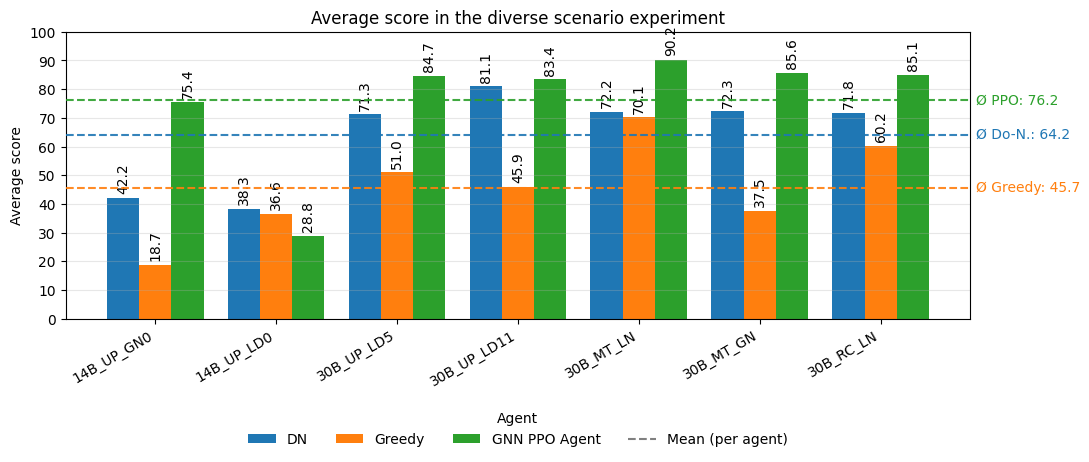
\includegraphics[width=1\textwidth]{images/experiments/total_scores/diverse_scenarios.png}
    \caption{Total score overview for the diverse scenario experiment, with average values of each agent}
    \label{fig:tot-score-diverse} 
\end{figure}

\paragraph{Modification of Generators and Loads.}
Figure \ref{fig:scenario-scores-14b-gnld-scaled} and \ref{fig:scenario-scores-30b-ld-scaled} show the results, for the power generation and consumption scaling experiment. For the load scaling in the 14-bus grid the three agents survived only in two of the three runs for more than one iteration. The last run got a score of zero, as no agent survived it. In the 14-bus scenarios the voltage violation mitigation of each agent is much lower than the scores of the 30-bus scenarios, while the overload mitigation scores are higher in the bus-14 scenarios. As for the survival, in all runs at least one agent has the maximum score of 100 or a score over 80, except for the second run in the scenario of increased load consumption in the 14-bus grid, where the scores are much lower. Also the \ac{ppo} agent usually has one of the highest scores in survival, but in all runs of the 14-bus increased load consumption scenario it reaches scores lower than the other agents. Also in the costs category this agent often has a low score, while the do-nothing agent achieved higher scores.

\paragraph{Modification through Maintenance and Line Capacity Reduction.}
Figure \ref{fig:scenario-scores-mnt} and \ref{fig:scenario-scores-rc} present the outcome of maintenance events and reducing the capacity of lines. The results are pretty similar in all three scenarios, with the \ac{ppo} agent achieving the best scores in all categories except costs, where the do-nothing got the highest scores. Just in the run of the line maintenance scenario the greedy agent has a maximum score, while performing with much lower scores in the other scenarios. In this scenario the do-nothing agent has a much lower value than usual in the costs category.

\subsubsection{Stress Test Results}
This experiment is made of three different experiments, with each different scaling of power generation, power consumption and line capacity. Table \ref{tab:exp_overview_stress} shows the average result over each of these tests. In general one can see, that the average scores, except in the line capacity scaling test, are much lower than in the previous experiments. In the generator and line capacity scaling trials the same pattern as in the other experiments can be seen, with the \ac{ppo} agent reaching the highest scores in all categories except the costs category. In the load scaling trial the do-nothing agent has the highest scores in all categories except of overload mitigation, where the \ac{ppo} agent has the highest score.

\begin{table}[htbp]
  \centering
  \caption{Comparison for the stress test experiment across all three scaling experiments}
  \label{tab:exp_overview_stress}
  \begin{tabular}{lrrr}
    \toprule
    Metric & Do-Nothing & Greedy & PPO \\
    \midrule
    \multicolumn{4}{l}{\textit{Generator Scaling}} \\
    Total Score & 33.39 & 17.30 & \textbf{40.21} \\
    Overload Mitigation & 54.35 & 43.20 & \textbf{59.02} \\
    Voltage Violation Mitigation & 13.19 & 10.70 & \textbf{21.23} \\
    Survival & 28.36 & 3.13 & \textbf{43.17} \\
    Costs & \textbf{46.99} & 21.20 & 31.65 \\
    \midrule
    \multicolumn{4}{l}{\textit{Load Scaling}} \\
    Total Score & \textbf{45.78} & 34.53 & 41.19 \\
    Overload Mitigation & 65.22 & 61.81 & \textbf{65.36} \\
    Voltage Violation Mitigation & \textbf{13.72} & 13.67 & 12.69 \\
    Survival & \textbf{48.15} & 26.62 & 40.39 \\
    Costs & \textbf{63.89} & 45.45 & 52.21 \\
    \midrule
    \multicolumn{4}{l}{\textit{Line Capacity Scaling}} \\
    Total Score & 72.00 & 58.79 & \textbf{84.88} \\
    Overload Mitigation & 44.32 & 51.78 & \textbf{78.23} \\
    Voltage Violation Mitigation & 62.71 & 25.75 & \textbf{90.59} \\
    Survival & \textbf{100.00} & 91.67 & \textbf{100.00} \\
    Costs & \textbf{61.91} & 40.28 & 41.43 \\
    \bottomrule
  \end{tabular}
\end{table}

\paragraph{Generator Stress Test.}
Figure \ref{fig:tot-score-gen-stress} shows the score distribution over all agents in the stress test experiment with the generator 0 from the 14-bus grid. In this stress test the agents did not survive any iterations for the highest generator scaling, thus leading to a low total score for each agent. While the do-nothing and greedy agent's scores decrease significantly over higher scaling, the score of the \ac{ppo} agent has a peak in the second highest scaling. Figure \ref{fig:scenario-scores-gn-stress} and \ref{fig:scenario-scores-14b-up-gn0} show also the average category score over each run for all scalings. For the highest scaling there are no plots, as the scores were zero. The increase of scoring for the \ac{ppo} is caused by a higher scoring in overload mitigation and survival for the second level of scaling. For the other agents the category scores lower between the first and second scaling. The greedy agent even reaches non-convergence for the third run of the second scaling.

\paragraph{Load Stress Test.}
Figure \ref{fig:tot-score-load-stress} shows the reached scores over all agents for the stress test experiment with the load 0 from the 14-bus grid. The scores of all three agents decline, as the scaling increases, with the do-nothing and \ac{ppo} agents having a strong decline after the first scaling. Figure \ref{fig:scenario-scores-ld-stress} and \ref{fig:scenario-scores-14b-up-ld0} show a more detailed scoring distribution of the individual runs in each scaling level. In the second and third level of scaling, no agent made any timestep converge during the third run of the scenario.

\paragraph{Line Capacity Stress Test.}
Figure \ref{fig:tot-score-line-cap-stress} shows the achieved scores over all agents in the stress test experiment with reduced capacity of lines in the 30-bus grid. In this experiment, the scores of each agent do not decline at all, remaining stable in their score ranges. Figure \ref{fig:scenario-scores-rc-stress} and \ref{fig:scenario-scores-rc} show the category score distribution over each level of line capacity reduction. The scores remain similar for the do-nothing and \ac{ppo} agents, while the greedy agent changes category scores, while still achieving similar average scores in each level. 

\subsection{Performance Test Results}\label{ssec:perf-test-result}
Table \ref{tab:exp_overview_performance} shows the results of the computational performance comparison between the greedy and \ac{ppo} agents. As explained in Section \ref{ssec:experiment-scenarios}, the do-nothing agent is not treated as a competing agent in this comparison because it serves as the computational reference baseline and performs no action-selection computation. The \ac{ppo} agent received a higher score than the greedy agent did in both the 14-bus and 30-bus scenarios, with scores close to the maximum in both grid sizes. The greedy agent on the other hand scored similarly in both grids, with a slightly higher score in the 30-bus grid.

\begin{table}[htbp]
\centering
\caption{Comparison of the agents in the performance test experiment}
\label{tab:exp_overview_performance}
\begin{tabular}{lrrr}
    \toprule
    Grid & Greedy & PPO \\
    \midrule
    14-bus & 63.65 & \textbf{98.68} \\
    30-bus & 66.67 & \textbf{99.34} \\
    \midrule
    Total & 65.16 & \textbf{99.01} \\
    \bottomrule
\end{tabular}
\end{table}

A closer look into the measured metrics of this experiment is illustrated in Table \ref{tab:exp_metrics_performance}. It demonstrates, that the \ac{ppo} agent has a faster runtime per timestep and a lower memory usage than the greedy agent, while the greedy agent always has a lower CPU usage than the \ac{ppo} agent. Notably, the runtime of the greedy agent increases considerably between the 14-bus and 30-bus grid, more than doubling, while the runtime of the \ac{ppo} agent stays nearly constant across both grid sizes. 

\begin{table}[htbp]
\centering
\caption{Measured average metric values for the performance test experiment}
\label{tab:exp_metrics_performance}
\begin{tabular}{llrr}
    \toprule
    Grid & Metric & Greedy & PPO \\
    \midrule
    \multirow{3}{*}{14-bus}
        & Runtime per timestep (s) & 3.98 & \textbf{1.32} \\
        & CPU usage (\%)           & \textbf{13.86} & 22.22 \\
        & Memory usage (\%)        & 27.22 & \textbf{11.08} \\
    \midrule
    \multirow{3}{*}{30-bus}
        & Runtime per timestep (s) & 8.47 & \textbf{1.44} \\
        & CPU usage (\%)           & \textbf{12.23} & 21.41 \\
        & Memory usage (\%)        & 26.61 & \textbf{11.55} \\
    \midrule
    \multirow{3}{*}{Total}
        & Runtime per timestep (s) & 6.23 & \textbf{1.38} \\
        & CPU usage (\%)           & \textbf{13.05} & 21.81 \\
        & Memory usage (\%)        & 26.91 & \textbf{11.32} \\
    \bottomrule
\end{tabular}
\end{table}





\section{Analysis and Interpretation}\label{sec:exp-analysis-interpretation}
This section provides a detailed analysis and interpretation of the experimental results presented in the previous section. 
First, Section \ref{ssec:metric-performance} takes a closer look at the individual metrics behind the category scores, explaining recurring patterns and problems in the agents' strategies. 
Building on this, Section \ref{ssec:influence-grid-size} examines how the size of the two utilised grid topologies affects the benchmark scores, independently of the specific grid modification applied. 
Section \ref{ssec:influence-modification} then discusses the effect of the individual grid modifications on scenario difficulty and the effects on the evaluated categories, using the do-nothing agent to isolate their impact. 
Section \ref{ssec:behaviour-stress} extends this analysis by examining the agents' behaviour under increasing stress levels for generator, load and line capacity scaling. 
Three representative runs are then examined in depth in Section \ref{ssec:case-studies} to explain notable differences between the do-nothing and \ac{ppo} agents. 
Section \ref{ssec:computational-performance} analyses the results of the performance test experiment, relating the measured runtime, CPU and memory usage to the architectural differences between the greedy and \ac{ppo} agents. 
Finally, Section \ref{ssec:agent-profiles} summarises all findings into a strength and failure profile for each agent, demonstrating how \benchmark can be used to systematically uncover both the capabilities and the shortcomings of \ac{rl}-based grid operation agents.

\subsection{Metric Performance}\label{ssec:metric-performance}
This subsection takes a closer look at the individual metrics evaluated by \benchmark, in order to explain the category-level scores discussed previously and to identify recurring patterns in the agents' strategies.

When looking at the metrics evaluated by \benchmark in Figure \ref{fig:metric-scores-overload} and \ref{fig:metric-scores-survival} one can see, that the \ac{ppo} agent achieved higher scores than the other agents in all metrics. This is due to the agent's goal in training, to reduce overloads in $N-0$ and to keep converging grid states. This aligns with the expectations formulated in Section \ref{ssec:exp-expectation}. However, the strategy chosen by the agent for some scenarios is problematic in real-world cases, as Figure \ref{fig:exp-grids-off} demonstrates for two scenarios in the 14- and 30-bus grid. To reduce the overloads of lines, the agent switches off the majority of the power grid, turning off every generator and only providing power to one load close to the external grid, by using the external grid as the only power source. This is a common problem with faulty reward functions, often called \textit{reward hacking} \cite{rewardHacking,openaiFaultyReward}. The agent tries to maximise its reward signal without achieving the intended goal for the decision problem. In this case the agent obtained a faulty reward, that only covers a part of important metrics for good power grid operation. It maximises overload mitigation and the avoidance of non-convergence, by making the problem easier to solve, disconnecting a majority of the power grid. However, this is not ideal for the actual problem of stable and ideal power grid operation, where the full power grid should work and receive power.

\begin{figure}[htp]
    \centering
    \begin{subfigure}[b]{0.53\textwidth}
        \centering
        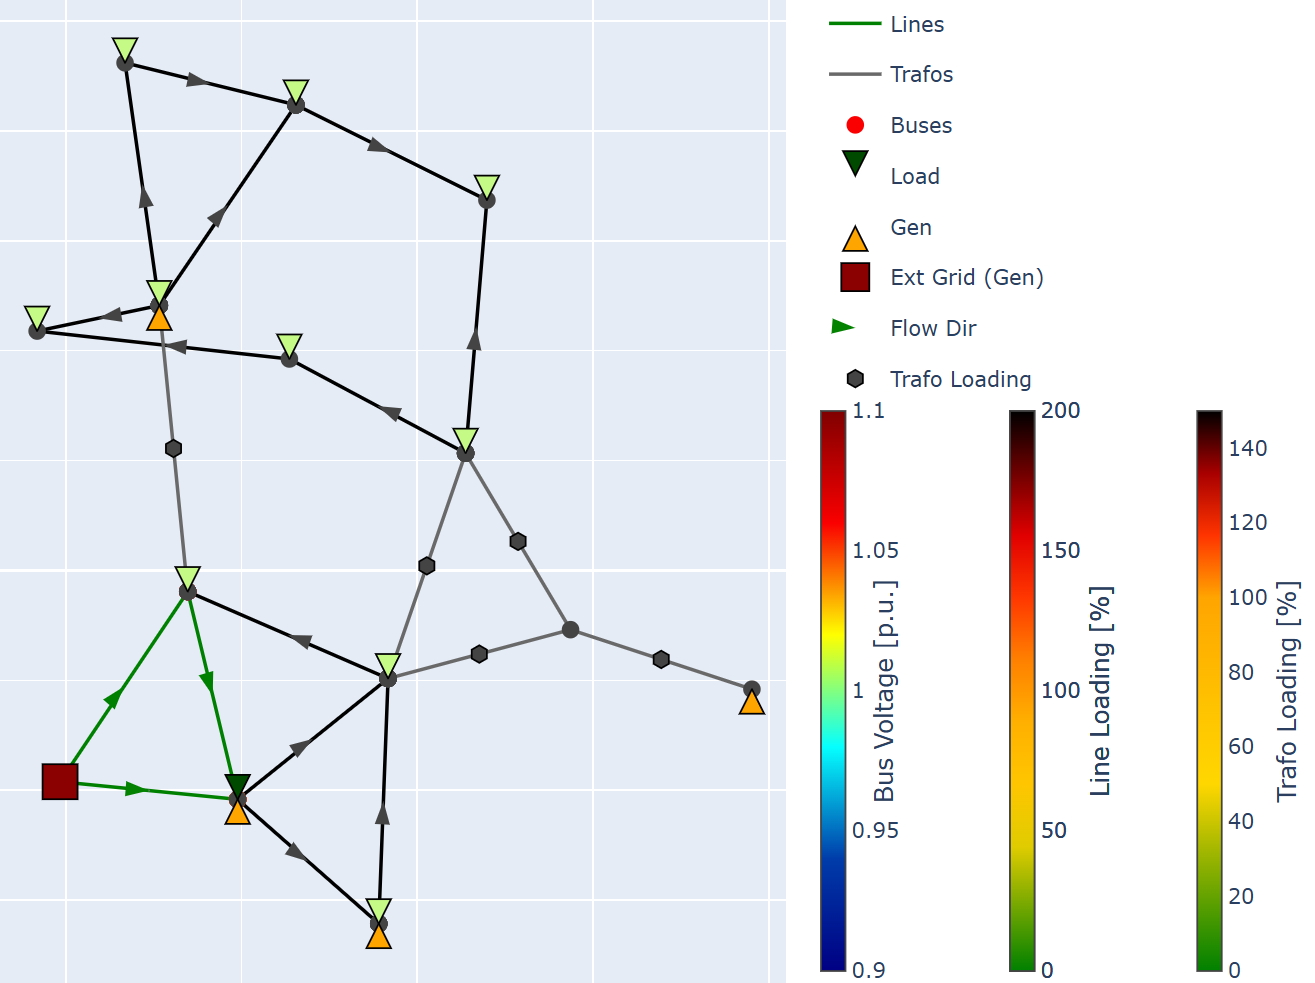
\includegraphics[width=\textwidth]{images/experiments/grids/14b_switched_off.png}
        \caption{Generator scaled 14-bus scenario, with every component disconnected, except the lines going to load 0 and 3}
        \label{fig:grid-14-off}
    \end{subfigure}
    \hfill
    \begin{subfigure}[b]{0.45\textwidth}
        \centering
        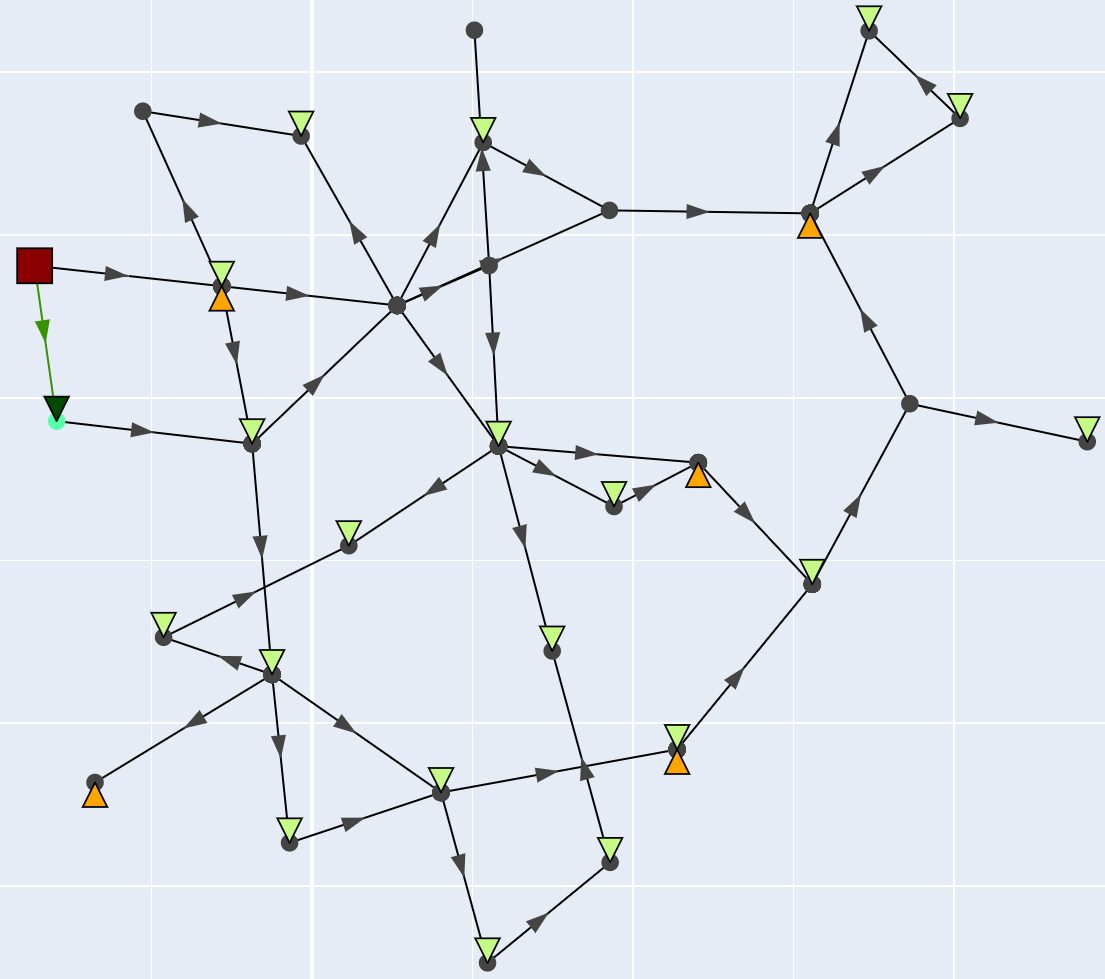
\includegraphics[width=\textwidth]{images/experiments/grids/30b_switched_off.png}
        \caption{Standard 30-bus scenario, with every component disconnected, except line 1 going to load 1}
        \label{fig:grid-30-off}
    \end{subfigure}
    \caption{Scenario showing the \ac{ppo} agent disconnecting most of the grid. The legend shown in \subref{fig:grid-14-off} applies to both subfigures}
    \label{fig:exp-grids-off}
\end{figure}

With the greedy agent the scores for $N-0$ overloads were also good, often reaching a score between the do-nothing and \ac{ppo} agents, however, it had problems with survival. Looking at the survival scores for each run, one can see them fluctuating between high and very low values. This is due to the exploitative nature of the greedy agent, only planning the current best step, but not looking ahead. This caused the agent to often do one substation-splitting action after another, changing the topology much more frequently than the \ac{ppo} agent. This caused the agent often to reach a non-converging state, where the simulation had to stop. 

An example of this behaviour can be observed in the standard, unmodified 30-bus scenario, shown in Figure \ref{fig:grid-30-greedy}. Here, the greedy agent repeatedly switches substations throughout the episode, in several instances even switching the same substation again in the very next timestep. As the external grid supplies by far the largest share of power to the 30-bus grid, these frequent and locally optimal, but globally uncoordinated, switching actions progressively worsen the loading of the transmission lines that carry power from the external grid to the highest-demand loads. This drives some line loadings above 130\% and causes bus voltages in the affected area to drop to as low as 15\% below the nominal level. As a result, the greedy agent survives only 26 of the 96 timesteps in this scenario. By contrast, the \ac{ppo} agent survives the full episode by resorting to its reward hacking strategy described above and shown in Figure \ref{fig:grid-30-off}, and the do-nothing agent also survives fully, though only after several lines are automatically put under maintenance due to excessive loading, cutting off the highest-demand load. Thus, both the \ac{ppo} and do-nothing agents stabilise the grid in this scenario only by sacrificing power delivery to parts of the grid, whereas the greedy agent fails to stabilise it at all through its uncoordinated switching behaviour.

\begin{figure}[htp]
    \centering
    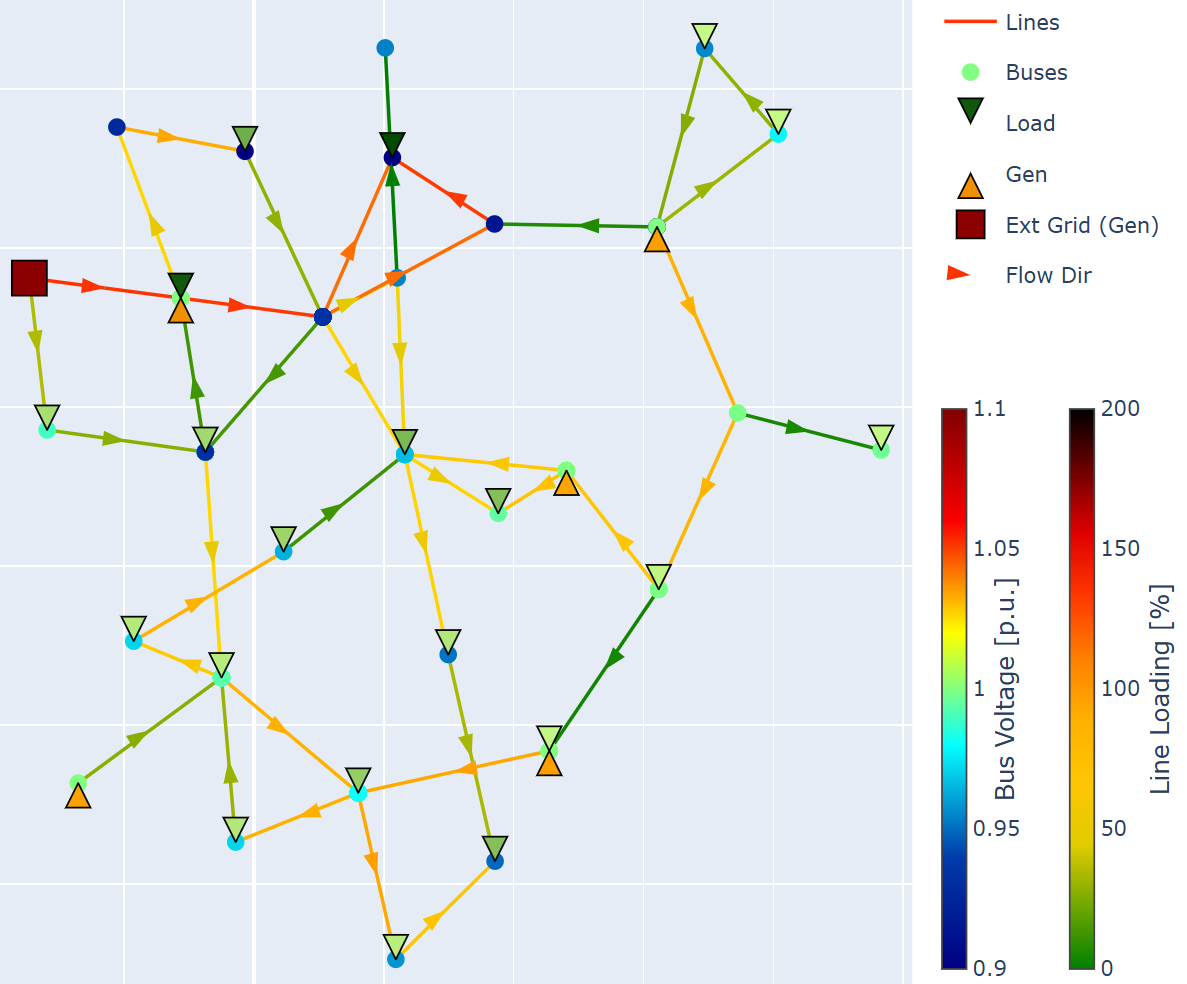
\includegraphics[width=0.57\textwidth]{images/experiments/grids/30b_original_greedy.png}
    \caption{Standard 30-bus scenario using the greedy agent, showing the last timestep before non-convergence was reached}
    \label{fig:grid-30-greedy} 
\end{figure}

In the overload mitigation category the do-nothing agent performed often worse than the other agents, due to not handling them at all. However, the survival score was almost as high as the one of the \ac{ppo} agent, which means that the experiments were not challenging enough, when it came to the survival category. Inaction was sufficient to avoid non-convergence for 70\% of the episode's timestep, on average.

For the voltage violation mitigation no agent had the goal to reduce them. This can be seen in Figure \ref{fig:metric-scores-voltage-violation} and in Table \ref{tab:agent_comparison}, as the average metric scores and category score for this aspect are much lower than the other metrics and categories. However, the \ac{ppo} agent had the highest scores, due to its strategy in some scenarios of disconnecting most of the power grid. 

When it comes to the cost category, it comes as no surprise, that the do-nothing has perfect scores for the metrics of substation changes and timesteps without actions. However, it is interesting that the \ac{ppo} agent learned to reduce the substation changes, while the greedy agent switches very frequently. While in some scenarios the \ac{ppo} agent only does one or two actions in total, the greedy agent often chooses different actions in each timestep. When it comes to load shedding, the \ac{ppo} agent performs very badly compared to the other agents. This is again due to its trained policy, which in many cases just delivers power to only one load close to the external grid, while not providing any power to the rest. 

\subsection{Influence of Grid Size}\label{ssec:influence-grid-size}
This subsection investigates the extent to which the size of the underlying power grid topology influences the benchmark scores, regardless of the specific grid modification applied. As the 14-bus and 30-bus grids differ substantially in terms of the number of components and electrical parameters, comparing their category scores directly may reveal systemic effects rooted in the grid structure itself rather than in the strategies employed by the agents.

As seen in Figure \ref{fig:exp-heatmap} and \ref{fig:bus-scores}, the category scores in the 14-bus power grid look different from the scores in the 30-bus grid. The 30-bus grid overall has higher scores, especially in survival and voltage violation mitigation. However, most of the scenarios that were compared, covered different grid modifications, making a direct comparison over all scenarios difficult. In general, each grid modification has much higher impact on the smaller grid, as the percentage of modified components is higher than in the bigger grid. If there are only three generators and eleven loads (see Figure \ref{fig:grid-14}), modifying one of them makes a significantly higher change, than changing one load out of twenty or putting one generator from five in maintenance.

Another difference that one can notice in all scenarios, is that the overload mitigation scores are lower in the 30-bus grid. When looking at the \textit{max\_i\_ka} values, it is clear why this happens. As explained in Section \ref{ssec:implementation-grid-mod}, \textit{max\_i\_ka} in pandapower defines the maximum allowed current (in kiloamperes), that can pass a transmission line or transformer. These values are at least 80 times higher in the 14-bus grid, than in the 30-bus grid. This extreme difference makes the lines in the 30-bus grid scenarios overload much faster, while they do not overload at all in the 14-bus grid. As the current can flow completely freely, this makes the 14-bus grid scenarios have other problems like power losses (regarding equation \eqref{eq:heat_power_dc}) and issues with nominal voltage levels (regarding equation \eqref{eq:high_voltage_low_current}). 

\subsection{Influence of Modifications}\label{ssec:influence-modification}
This subsection analyses the various grid modifications introduced in Section \ref{ssec:implementation-grid-mod} and their impact on the difficulty of a scenario. As the do-nothing agent does not perform any corrective actions, its scores can be used to isolate the impact of each modification on the power grid without the influence of an agent's strategy. The examination includes the effects of load and generator scaling, generator maintenance and line capacity scaling and maintenance.

\subsubsection{Load Scaling}
When looking at Figure \ref{fig:tot-score-diverse}, the load scaling in the 14-bus grid had the biggest impact. As seen in \ref{fig:scenario-scores-14b-up-ld0}, one of the three runs did not converge for any iteration and the second run got low survival scores overall. Also voltage violation mitigation has very low scores in this scenario, as shown in Figure \ref{fig:grid-14-load-inc} with the buses often being around 10\% over the nominal voltage level (visible in the colour scale in red; the darker the red, the higher the level). 

\begin{figure}[htp]
    \centering
    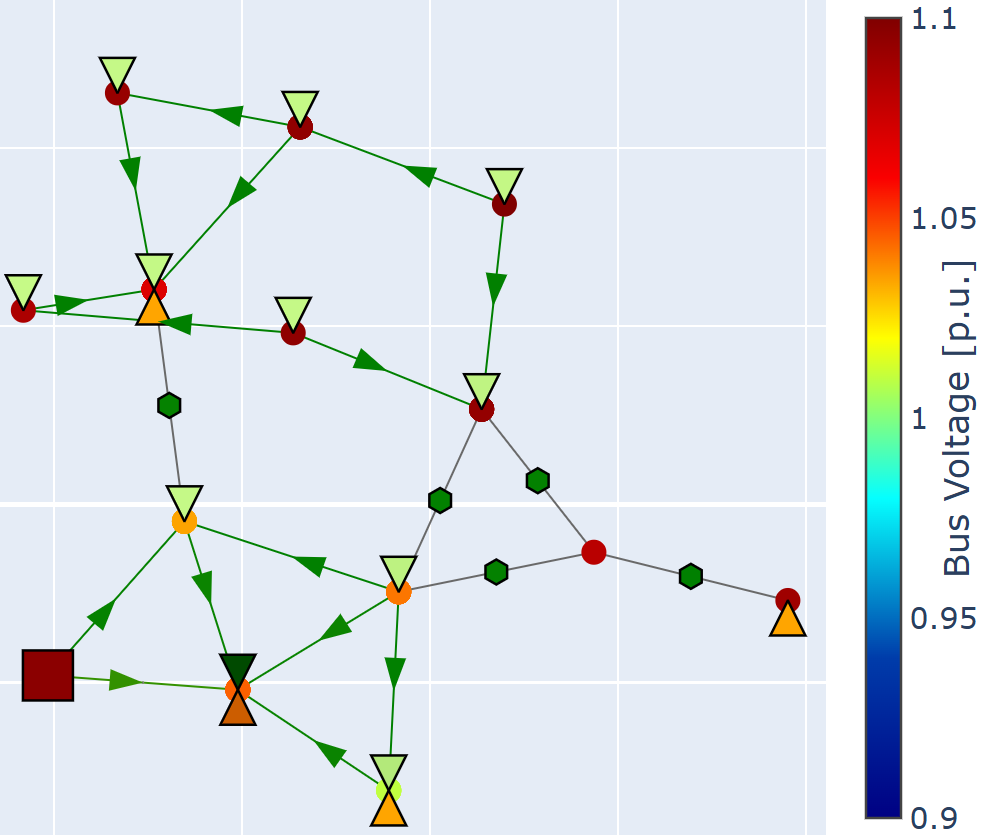
\includegraphics[width=0.5\textwidth]{images/experiments/grids/14b_load_inc.png}
    \caption{Bus voltages mostly above nominal level for the do-nothing agent in the 14-bus scenario with increased consumption at load 0}
    \label{fig:grid-14-load-inc} 
\end{figure}

For the 30-bus grids the upscaled load consumption in single loads caused the lines around the load always to be put into maintenance, due to the high line loadings. Figure \ref{fig:grid-30-load-inc} shows it for one run of the scaling of load 5, however, the results were the same in the other runs and with load 11 too. Always the lines connected to, or close to the scaled load reached overloadings. This made the scaled loads get no power at all, leading to poor scores in the costs and overload mitigation category, as Figure \ref{fig:scenario-scores-30b-up-ld5} and \ref{fig:scenario-scores-30b-up-ld11} show. In the 14-bus scenario with load scaling the lines did not have overloading issues. This is due to the \textit{max\_i\_ka} values in the transmission lines, explained in Section \ref{ssec:influence-grid-size}.

\begin{figure}[htp]
    \centering
    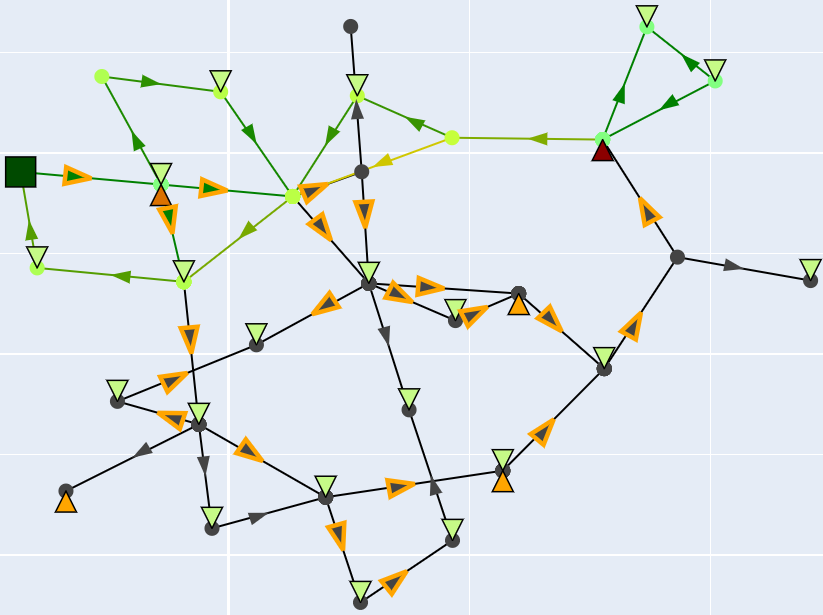
\includegraphics[width=0.54\textwidth]{images/experiments/grids/30b_load_inc.png}
    \caption{Lines in maintenance around load 5, for the do-nothing agent in the 30-bus scenario with increased consumption at load 5}
    \label{fig:grid-30-load-inc} 
\end{figure}

\subsubsection{Generator Scaling and Maintenance}
When it comes to increased power generation in the 14-bus scenario, it is visible, that it had an impact on the do-nothing and greedy agents' scores, achieving similar results to those of the load scaling scenario. When looking at Figure \ref{fig:scenario-scores-14b-up-gn0} it is clear, that both the do-nothing and the greedy agent struggled to maintain convergence and to lower the voltage violations. This is again due to the bus voltages, but contrary to the increased load, increasing the generation lowered the bus voltages. This is shown in Figure \ref{fig:grid-14-gen-inc}, where most buses are 10\% or more below the nominal voltage level (visible in the colour scale in blue; the darker the blue, the lower the level). 

\begin{figure}[htp] 
    \centering
    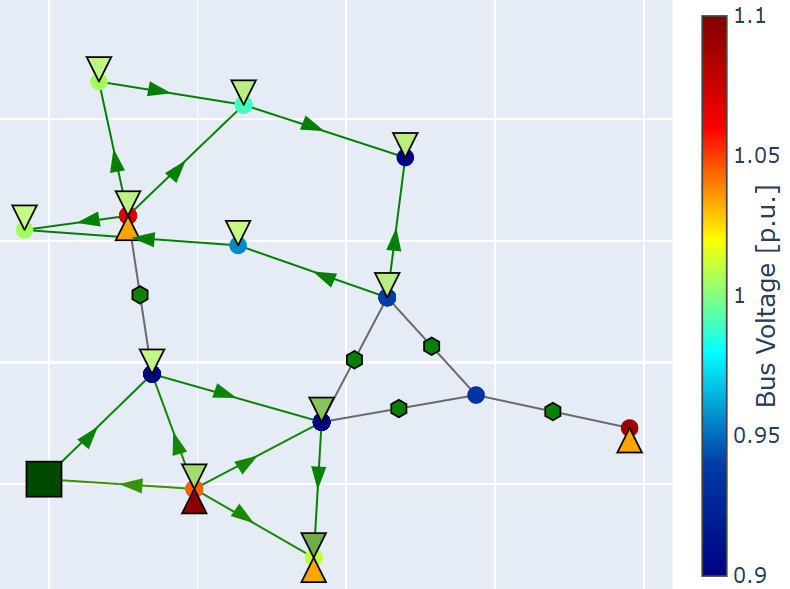
\includegraphics[width=0.53\textwidth]{images/experiments/grids/14b_gen_inc.png}
    \caption{Bus voltages mostly below nominal level for the do-nothing agent in the 14-bus scenario with increased production at generator 0}
    \label{fig:grid-14-gen-inc} 
\end{figure}

When it comes to the generator maintenance, that was applied in one of the 30-bus scenarios, the results are nearly identical to the normal 30-bus scenario. When looking at Figure \ref{fig:scenario-scores-30b-orig} and \ref{fig:scenario-scores-30b-mt-gn}, the scores are almost the same for each agent and category. Even when looking at the replay data, presented in Section \ref{ssec:replay-data}, the graphs of both scenarios look identical. The only difference is, that the external grid has to be used much more in the case of the generator maintenance, to make up for the missing power generation from the generator that is under maintenance. Other than that the same three lines overload and the rest of the grid runs relatively stable, making the do-nothing agent never reach a non-converging state. 

\subsubsection{Line Capacity Scaling and Maintenance}
For the grid modification of the line capacity scaling and line maintenance, the results behave very similarly in both modifications. For the do-nothing the same scores can be measured in all categories, as seen in Figure \ref{fig:scenario-scores-30b-mt-ln} and \ref{fig:scenario-scores-rc}. Due to the changes in the edges of the power grid, the grid goes into a complete shutdown at the 26th timestep in both scenarios. In both of them the shutdown is caused by a chain reaction, where multiple transmission lines reach an overloading over 150\% in the 25th step, causing them to be put under maintenance in the 26th timestep. After this step, all the lines connected to the external grid are under maintenance, removing a power source delivering around 250 MW of energy. Figure \ref{fig:grid-30-line-rc} demonstrates the 25th, showing the overloaded lines in a red to black colour, and 26th step, with overloaded lines marked with an orange arrow. The lines that are already overloaded in the 25th step are the ones that have been reduced in line capacity and thus overloaded in the first 20 steps. Making the grid completely powerless has a positive effect on the survival score, as when there is no power, the states always converge. The overload mitigation scores, however, are very low in these scenarios, due to constant overloadings.

\begin{figure}[htp]
    \centering
    \begin{subfigure}[b]{0.48\textwidth}
        \centering
        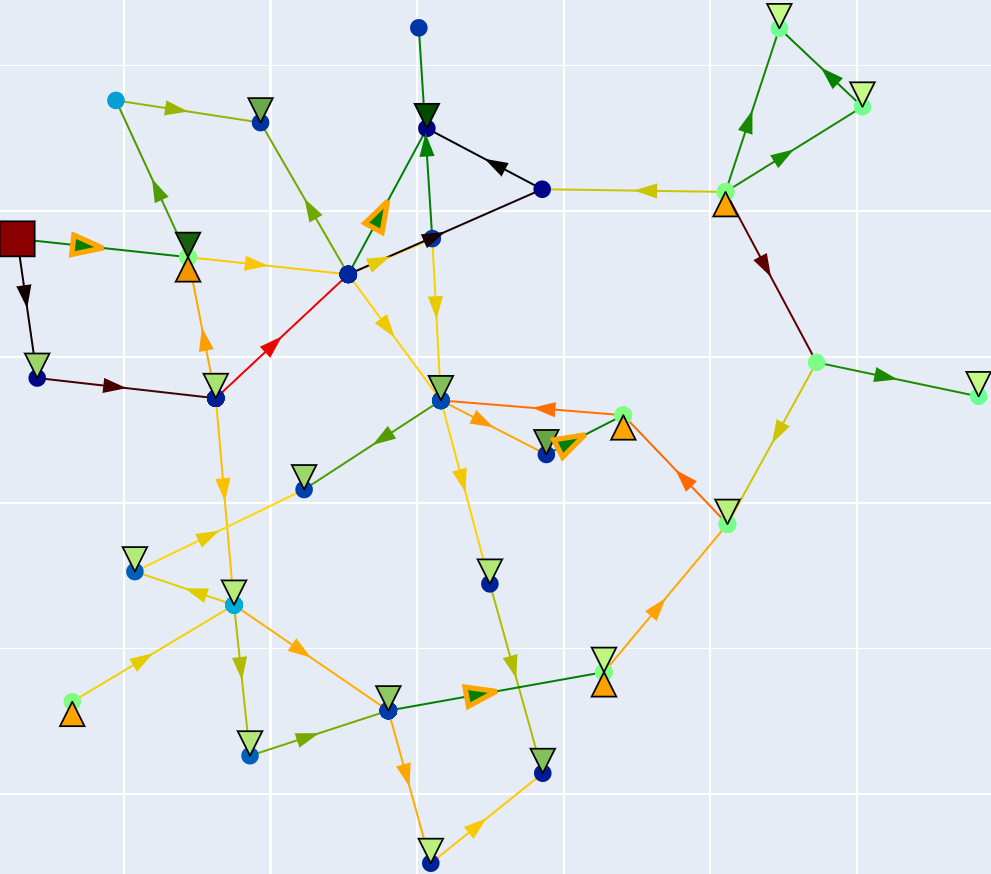
\includegraphics[width=\textwidth]{images/experiments/grids/30b_line_event_bf.png}
        \caption{25th timestep}
        \label{fig:grid-30-line-rc-bf}
    \end{subfigure}
    \hfill
    \begin{subfigure}[b]{0.48\textwidth}
        \centering
        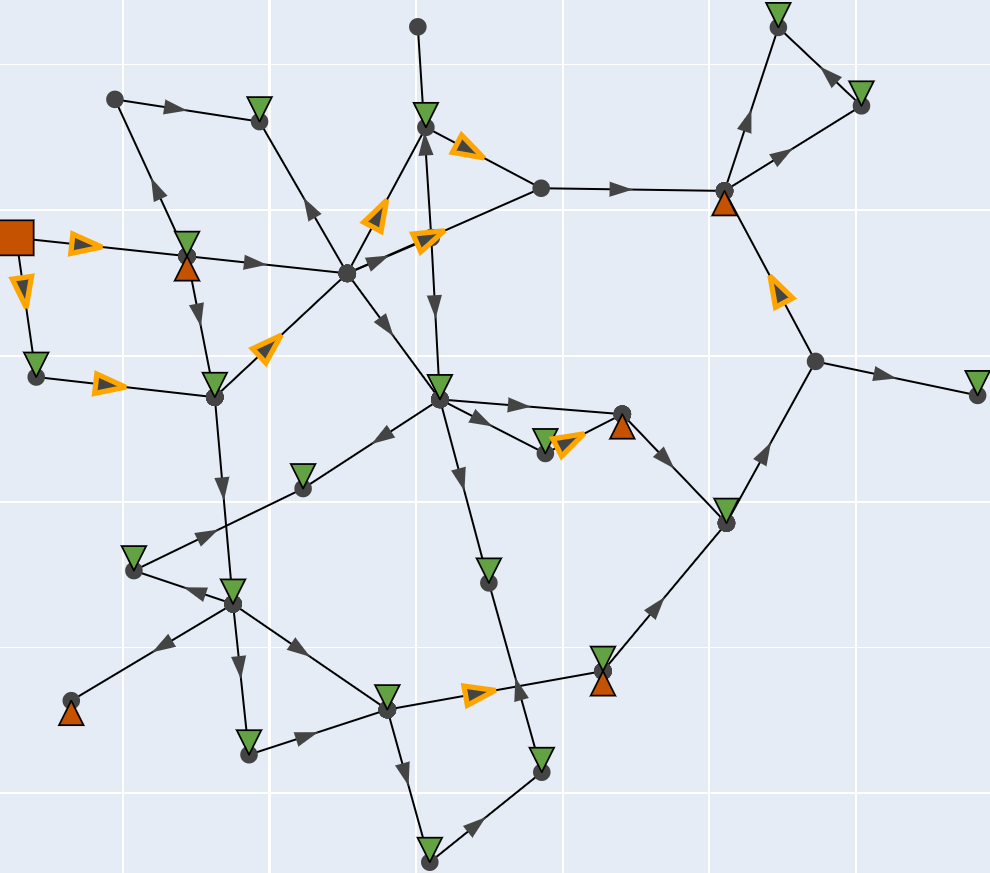
\includegraphics[width=\textwidth]{images/experiments/grids/30b_line_event_af.png}
        \caption{26th timestep}
        \label{fig:grid-30-line-rc-af}
    \end{subfigure}
    \caption{Complete powerless grid for the do-nothing agent in the 30-bus scenario with reduced line capacity}
    \label{fig:grid-30-line-rc}
\end{figure}


\subsection{Behaviour Under Increasing Stress}\label{ssec:behaviour-stress}
This subsection examines the results of the three stress tests conducted in the experiments, in which the generator, load and line capacity modifications are scaled up over multiple levels, to assess how the agents behave when scenarios diverge further from the nominal operating point. Comparing the category scores across these increasing scaling levels allows conclusions to be drawn about the robustness of each agent's strategy.

\subsubsection{Generator Stress Test}
For the generator stress test the do-nothing and greedy agents behaved as expected in Section \ref{ssec:exp-expectation}, as Figure \ref{fig:tot-score-gen-stress} shows. Both agents decline in performance over each increased level of difficulty. For the \ac{ppo} agent however, it is interesting to see, that it increased in scoring for the second scaling of the generator. In the second trial of this stress test, the agent reached perfect survival scores, while it achieved worse scores in the first scaling. When looking at Table \ref{tab:training-results} one can see, that the agent obtained more than double of the cumulative reward for the best training iteration for the second scaling compared to the first, lower scaling. Thus it was trained much better in $N-0$ overloads and grid convergence, and knew better actions. In the highest scaling it received the lowest cumulative reward over all trained scenarios, which explains the bad performance in the scenario. However, the third level of scaling is impossible to stabilise and get a score higher than zero, as it is already too unstable in the first profile step.  

\subsubsection{Load Stress Test}
The load stress test behaves as expected for all three agents, as Figure \ref{fig:tot-score-load-stress} demonstrates. However, the decline of the \ac{ppo} agent is worth noting, as it does very steeply between the first and second scaling, but not much for the last scaling. Even looking at the individual runs in Figure \ref{fig:scenario-scores-14b-up-ld0} and \ref{fig:scenario-scores-14b-up-ld0-high}, both scaling had similar category scores. This is not represented in the training values, as the second scaling had more than double of the cumulative reward compared to the third scaling. When looking at the actions in both scaling levels, the agent is always doing just one splitting action in the beginning and then no or just one action through the rest of the episode. With this it almost behaves like a do-nothing agent, not interacting much with the grid. With more tuning and training and a better reward function the agent could find better actions to interact with the grid.

\subsubsection{Line Capacity Stress Test}
The line capacity test resulted unexpectedly compared to the expectations formulated in Section \ref{ssec:exp-expectation}. The agents achieved almost constantly the same scores over each scaling, as Figure \ref{fig:tot-score-line-cap-stress} reveals. The reason for the same scores, is that the runs of each scaling behave exactly the same. As explained in Section \ref{ssec:influence-modification}, the second level of line capacity reduction made the grid turn into a powerless state in the 26th step. This event happens in the same way and at the same timestep for the other scaling of line capacity. For this reason the scores are all high, even in the highest scaling. With the grid being out of power, the grid stability can not become worse.

\subsection{Case Studies - Do-nothing vs. PPO}\label{ssec:case-studies}
In most scenarios of the experiments the \ac{ppo} agent achieved a higher or equal survival score than the do-nothing agent. However, there were a few cases, where the do-nothing agent beat the \ac{ppo} agent in convergence, even though the \ac{ppo} was trained to avoid it. In this section, three case studies are analysed more in depth, each of them focussing on one run of a specific scenario. In the first case study, the run at index 21120 (day 220) of the unmodified 14-bus grid is looked at. Here the do-nothing agent slightly outperformed the \ac{ppo} agent in the survival score, maintaining convergence a couple of timesteps longer. In the second case study, the second run at index 18240 (day 190) of the lowest generator stress test scenario is observed. This has the highest difference in grid convergence, as the do-nothing survived the full episode, while the \ac{ppo} agent only survived around 30\% of it. The final study looks at an opposite case. It compares the next level of the generator stress test, by looking at the same index as in the second case study. Here, even though it is the same profile day as in the second study with just more generator scaling, the scores in survival between the do-nothing and \ac{ppo} agents are swapped, with the \ac{ppo} agent clearing the episode while maintaining convergence.  

\subsubsection{Initial Observations} 
Firstly, for all the case studies, the actions are replayed, using the replay data presented in Section \ref{ssec:replay-data}. In general it stands out that the \ac{ppo} agent does just one or two actions directly in the first steps, and then it chooses no action, that changes the power grid. In Figure \ref{fig:grids-case-study}, one can see the obtained partial graphs of the grid, after the \ac{ppo} agent's actions have been implemented. For the first and second study, the agent does only one action, on one of the substations connected to one of the five transformers of the 14-bus grid. This does not seem to make a big difference, as the power grid's power flow just slightly changed, but all components still have paths between each other. In the third case study the agent splits the two substations, that are connected with a transmission line with the external grid, shutting off the rest of the grid and only providing power to the first load. The exact outcome is shown in Figure \ref{fig:grid-14-off}, which has been explained previously as being one of the agent's faulty strategy. Comparing this scenario to the others, it explains how the agent maintained convergence much longer in this scenario, compared to the other scenarios, where the agent did not follow this strategy. 

For the first study, the do-nothing performs a few steps more, than the \ac{ppo} agent. The action chosen by the \ac{ppo} probably brought a slight disadvantage to the agent, making it slightly less stable, in an already unstable grid, where inaction brings a quick failure of the grid. For the second study the do-nothing agent does not reach any non-converging grid states and finishes the whole episode, unlike the third study case, where the simulation ends after roughly a third of the episode. The changes in performance between the two cases is due to the increase of power production of generator 0. 

\subsubsection{Cross-Case Diagnostics} 
Now having compared each study, by only looking at the agents separately, a closer look at the two agents' performance is needed. For the 14-bus, as already discovered in \ref{ssec:influence-modification}, the lines do not have many issues with getting overloaded, thus a lot of current can pass through them. When performing a more detailed diagnosis of the simulations using pandapower's diagnostics functionality, warnings were issued for high \textit{vk\_percent} values (known as short-circuit voltage \cite{pandapower_docs} or percentage impedance \cite{impedance_percentage}) inside the transformers. This value controls how much a transformer resists the flow of power, in a similar way to resistance in an electrical circuit \cite{impedance_percentage}. In practice, this value is normally between 4\% and 15\%, and pandapower's diagnostic tool flags anything above 15\% as implausible \cite{pandapower_docs}. In the network model used for this thesis, all five transformers of the 14-bus grid had values above 1000\%. A higher value results in a greater voltage drop as more power flows through it \cite{impedance_percentage,transformer_impedance_regulation}. In these scenarios, the bus voltages around the transformers drop very low, sometimes even a voltage drop of up to 20\% compared to the nominal bus voltage. As explained in Section \ref{sssec:const_character_pg}, the voltages should remain within 10\% of the nominal value, to ensure a stable grid. These low values are explained, by the extreme \textit{vk\_percent} values in all of the transformers. These voltage drops make the grid extremely unstable. 

In the first two case studies, the \ac{ppo} agent chooses an action, which splits substations directly at one of the transformers. This causes changes in the current of the transformers, in an already highly unstable grid. For this reason, in the simulation of the \ac{ppo} agent, the bus voltages of the buses at the transformers are lower than the ones of the do-nothing agent. This makes the runs of the \ac{ppo} agent stop sooner than the ones of the do-nothing agent. On the third case study, however, the agent cuts off every part of the grid, except for the buses connected to the external grid and the load connected to it (as seen in Figure \ref{fig:grid-14-off}). This means, that the transformers are also not part of the grid, where power flows. This solves the instability caused by the transformers, making the \ac{ppo} agent go through the whole run, unlike the do-nothing agent that reaches non-convergence in the beginning of the run.


\subsection{Computational Performance}\label{ssec:computational-performance}
This subsection analyses the results of the performance test experiment presented in Section \ref{sec:experiment-results}, relating the measured runtime, CPU and memory usage back to the architectural differences between the greedy and \ac{ppo} agents discussed in Section \ref{ssec:custom-agent-setup}.

As expected, the \ac{ppo} agent is considerably faster than the greedy agent in both grid sizes. This is explained by the fundamental difference in how both agents select an action. While the greedy agent must simulate the resulting reward for every candidate switching action at every timestep, the trained policy of the \ac{ppo} agent maps a grid state directly to a single action. This difference becomes more obvious as the grid size increases. While the runtime per timestep of the \ac{ppo} agent remains almost constant between the 14-bus and 30-bus grid (1.32s vs. 1.44s), the runtime of the greedy agent more than doubles (3.98s vs. 8.47s), confirming the expectation formulated in Section \ref{ssec:exp-expectation} that the runtime advantage of the \ac{ppo} agent would be more significant in the larger grid, due to its larger action space.

The memory usage follows a similar pattern, with the \ac{ppo} agent using less than half the memory of the greedy agent in both grid sizes. This is likely because the greedy agent needs to keep multiple simulated copies of the grid state in memory simultaneously, one for each candidate action being evaluated, while the \ac{ppo} agent only performs a single forward pass through its policy network per timestep to decide an action.

The CPU usage, however, shows the opposite trend, with the \ac{ppo} agent consistently using more CPU than the greedy agent. This is presumably due to the batched matrix operations required for the neural network inference, which can utilise multiple CPU cores in parallel, whereas the sequential, one-by-one evaluation of candidate actions by the greedy agent does not fully utilise the available cores despite requiring a longer overall runtime. This illustrates, that the runtime advantage of the \ac{ppo} agent does not come without any computational trade-off, shifting resource demand from runtime and memory towards CPU utilisation. However, if the greedy agent were to parallelise its evaluation of candidate actions across more CPU cores, this would increase its CPU usage while also reducing its runtime per timestep. The user would then have to weigh the trade-off between a lower runtime and a lower CPU usage, depending on the computational resources available.



\subsection{Agent Behaviours and Profile}\label{ssec:agent-profiles}
Based on the observations from the previous subsections, this final subsection summarises the results to create a strengths and weaknesses profile for each of the three agents. This provides a concise summary of each agent's typical behaviour and demonstrates how the measured metrics and categories of \benchmark can be used to identify the capabilities and shortcomings of a power grid operation agent. Table \ref{tab:agent-profiles} summarises the discussed strengths and weaknesses of the three agents identified in the previous analysis. Each agent is then discussed in more detail below.

\begin{table}[htp]
    \centering
    \caption{Strengths and weaknesses of the evaluated agents}
    \label{tab:agent-profiles}
    \begin{tabularx}{\textwidth}{l X X}
        \toprule
        \textbf{Agent} & \textbf{Strengths} & \textbf{Weaknesses} \\
        \midrule
        Do-nothing &
        Perfect cost scores in action metrics (no actions at all); often high survival; no unintended load shedding &
        No overload or voltage violation mitigation; fails under increased stress \\
        \addlinespace
        Greedy &
        Decent $N-0$ overload mitigation, often between do-nothing and \ac{ppo}; reacts immediately to overloads &
        Highly unstable survival scores due to lack of lookahead; frequent substation switching (worst action metric scores); decline under stress; low computational efficiency \\
        \addlinespace
        \ac{ppo} &
        Highest scores in most metrics; learned to minimise substation changes; good in mitigating overloads and voltage violations; best convergence in several scenarios, even under stress; fast action computation &
        Reward hacking (disconnects most of the grid); lots of load-shedding; voltage improvements only a side effect of shutdown; can destabilise fragile grids via ill-timed splitting actions \\
        \bottomrule
    \end{tabularx}
\end{table}

\subsubsection{Do-nothing Agent}
\textbf{Strength Profile:} The do-nothing agent's main strength lies in its predictability and perfect cost scores, as it never performs any switching action (see Table \ref{tab:agent_comparison}). In scenarios not too far from the nominal operating point, inaction alone was sufficient to avoid non-convergence for a large share of the episode, as reflected in the survival scores of Figure \ref{fig:metric-scores-survival}. In individual case studies it even outperformed the trained \ac{ppo} agent in survival, most notably in the lowest generator stress test (Figure \ref{fig:tot-score-gen-stress}), where it completed the full episode while \ac{ppo} survived only about a third of it.

\textbf{Failure Profile:} Its main weakness lies in its design, which does not allow for any actions on the grid. Because of this it does not react to problems, resulting in low scores for overload and voltage violation mitigation across many scenarios. This is shown in the average metric scores in Figure \ref{fig:metric-scores-overload} and \ref{fig:metric-scores-voltage-violation} and also in the average scores shown in Table \ref{tab:agent_comparison}. As soon as a modification pushes the grid noticeably away from its nominal state, performance collapses, as shown in the load and generator stress tests (Figures \ref{fig:tot-score-load-stress} and \ref{fig:tot-score-gen-stress}).

\subsubsection{Greedy Agent}
\textbf{Strength Profile:} The greedy agent's strength is its fast, reactive overload mitigation, often scoring between the do-nothing and \ac{ppo} agents in the $N-0$ category, as seen in Figure \ref{fig:metric-scores-overload}. By always selecting the locally optimal action, it resolves immediate line overloads that the do-nothing agent does not handle.

\textbf{Failure Profile:} It is important to note that the scenario selection process described in Section \ref{ssec:experiment-scenarios} deliberately favoured profile days on which the greedy agent scored lower than the do-nothing agent. As a result, the failure profile presented here is likely more pronounced than it would be on an unfiltered, representative sample of grid conditions, and should be interpreted as an illustration of the greedy agent's worst-case behaviour rather than its typical performance across arbitrary scenarios. 
With this in mind, its short-sighted, purely exploitative strategy without lookahead is its main weakness. Performing one substation-splitting action after another causes frequent, large topology changes, leading to highly fluctuating grid stability and thus survival scores, as seen in Figure \ref{fig:metric-scores-survival}. This also leads to the worst scores in the cost category, when it comes to metrics that measure the frequency of actions. Furthermore, its performance deteriorates, when increasing the stress level, as Figure \ref{fig:tot-score-gen-stress} and \ref{fig:tot-score-load-stress} show, without any adaptive improvement. Additionally, it is not efficient in computational performance, needing a lot of time and memory in action decision. 

\subsubsection{PPO Agent}
\textbf{Strength Profile:} The \ac{ppo} agent achieved the highest overall scores across most of the metrics, particularly overload mitigation and survival, as Figure \ref{fig:metric-scores-overload} and \ref{fig:metric-scores-survival} and Table \ref{tab:agent_comparison} show. This confirms that its training objective of reducing $N-0$ overloads and avoiding non-convergence, was learned successfully. It also acts efficiently, often needing only one or two actions per episode, yielding better cost scores than the greedy agent. In several scenarios it kept the grid converging notably longer than the other two agents, for instance in the second generator stress test scaling, as shown in Figure \ref{fig:tot-score-gen-stress}. Additionally, in the computational efficiency test it achieved high scores, keeping the average runtime constant as grid size increases. 

\textbf{Failure Profile:} The agent's central weakness is in its policy, which uses a form of reward hacking. In multiple scenarios it learned to disconnect nearly the entire grid, supplying only a single load near the external grid to trivially avoid overloads and non-convergence, as illustrated in Figure \ref{fig:exp-grids-off}. This produces the worst load-shedding scores of all agents, as Figure \ref{fig:metric-scores-costs} shows. Moreover, its seemingly strong voltage-violation score, documented in Figure \ref{fig:metric-scores-voltage-violation}, is merely a side effect of powering down most of the grid rather than an active mitigation strategy. When it instead interacts through substation-splitting actions that do not disconnect most of the grid, as shown in Figure \ref{fig:grids-case-study}, it can occasionally worsen an already unstable state, causing earlier failure than a fully passive do-nothing agent. In certain situations involving increased stress, such as during the load stress test, the learned policy can also become almost completely passive, not improving the grid's state at all.